\documentclass[a4paper, 14pt]{extarticle}

\usepackage[T2A]{fontenc}
\usepackage{natbib}
\usepackage{graphicx}
\usepackage[english, russian]{babel}
\usepackage{fontspec}
\usepackage{amsmath}
\usepackage{amsfonts}
\usepackage{amssymb}
\usepackage{amsthm}
\usepackage{mathtools}
\usepackage{mathrsfs}
\usepackage{icomma}
\usepackage{fullpage}
\usepackage{ulem}
\usepackage{setspace}
\usepackage{listings}
\usepackage{indentfirst}
\usepackage[left=2cm,right=1.5cm,top=2cm,bottom=2cm]{geometry}
\usepackage{xcolor}
\usepackage{float}
\usepackage{csquotes}
\usepackage{hyperref}
\usepackage{graphics}



\definecolor{urlcolor}{HTML}{0000FF} % цвет гиперссылок
\definecolor{linkcolor}{HTML}{000000} % цвет гиперссылок
\hypersetup{pdfstartview=FitH, linkcolor=linkcolor, urlcolor=urlcolor, colorlinks=true}


\setmainfont{Times New Roman}
\setlength{\parindent}{5ex}
\setlength{\parskip}{1em}
\renewcommand{\baselinestretch}{1}

\graphicspath{{images/}}


\definecolor{buzzlightyear}{HTML}{8757A5}
\definecolor{grass}{HTML}{738D06}
\definecolor{literal}{HTML}{F18A2B}
\definecolor{commentcolor}{HTML}{8E908B}

\lstdefinestyle{habrstyle}{
    backgroundcolor=\color{white},
    commentstyle=\color{commentcolor},
    keywordstyle=\bfseries\color{buzzlightyear},
    numberstyle=\tiny\color{commentcolor},
    stringstyle=\color{grass},
    basicstyle=\ttfamily\footnotesize,
    breakatwhitespace=false,
    breaklines=true,
    captionpos=b,
    keepspaces=true,
    numbers=left,
    numbersep=5pt,
    showspaces=false,
    showstringspaces=false,
    showtabs=false,
    tabsize=4
}

\lstset{style=habrstyle}

\begin{document}
    % НАЧАЛО ТИТУЛЬНОГО ЛИСТА
    \begin{center}
        \begin{center}
            \hfill \break
            \normalsize{Санкт-Петербургский государственный политехнический}\\
            \normalsize{университет Петра Великого}\\
            \hfill \break
            \normalsize{\textbf{Высшая школа интеллектуальных систем и}}\\
            \normalsize{\textbf{суперкомпьютерных технологий}}\\
            \hfill \break
            \hfill \break
            \hfill \break
            \normalsize{Лабораторная работа}\\
            \hfill \break
            \normalsize{\LARGE Дифференцирование и интегрирование}\\
        \end{center}
        \hfill \break
        \hfill \break
        \hfill \break
        \hfill \break
        \hfill \break
        \hfill \break
        \hfill \break
        \hfill \break
        \hfill \break
        \hfill \break
        \begin{tabbing}
            Выполнил студент гр. 3530901/80201 \`И.С. Иванов\\
            \\
            Преподаватель: \`Н.В. Богач\\
        \end{tabbing}
        \hfill \break
        \hfill \break
        \hfill \break
        \hfill \break
        \begin{center}
            Санкт-Петербург\\
            2021
        \end{center}
        \thispagestyle{empty}
    \end{center}
    % КОНЕЦ ТИТУЛЬНОГО ЛИСТА

    % ОГЛАВЛЕНИЕ
    \newpage
    \tableofcontents

    % СПИСОК ИЛЛЮСТРАЦИЙ
    \newpage
    \listoffigures

    % СПИСОК ЛИСТИНГОВ
    \newpage
    \lstlistoflistings

    \newpage


    \section{Упражнение №1}
    \label{sec:1}

    В первом упражнении необходимо изучить примеры из файла \texttt{chap09.ipynb}.
    Далее необходимо заменить пилообразный сигнал на непериодические данные \texttt{Facebook} в примере нарастающей суммы.

    Создадим сигнал.

    \begin{lstlisting}[language=Python, caption= Создание сигнала facebook, label={lst:make_signal_fb}]
        df = pd.read_csv('Res/FB_2.csv', header=0, parse_dates=[0])
        ys = df['Close']
        in_wave = Wave(ys, framerate=1)
        in_wave.plot()
        decorate(xlabel='Time (s)')
    \end{lstlisting}

    \begin{figure}[H]
        \centering
        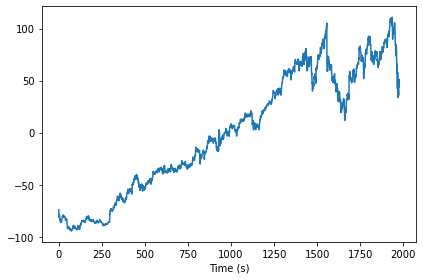
\includegraphics[width=0.8\linewidth]{signal_facebook}
        \caption{Сигнал Facebook}
        \label{fig:signal_facebook}
    \end{figure}

    Построим спектр.

    \begin{figure}[H]
        \centering
        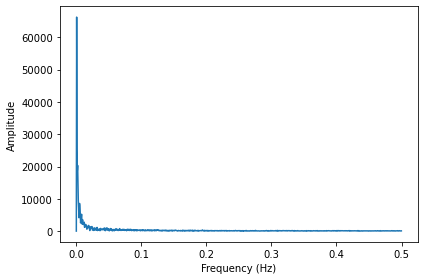
\includegraphics[width=0.8\linewidth]{facebook_spectrum}
        \caption{Спектр сигнала Facebook}
        \label{fig:facebook_spectrum}
    \end{figure}

    Получим выходной сигнал, который является совокупной суммой входных сигналов, и его спектр

    \begin{lstlisting}[language=Python, caption= Получение выходного сигнала, label={lst:make_output}]
        out_wave = in_wave.cumsum()
        out_wave.unbias()
        out_wave.plot()
        decorate(xlabel='Time (s)')
    \end{lstlisting}

    \begin{figure}[H]
        \centering
        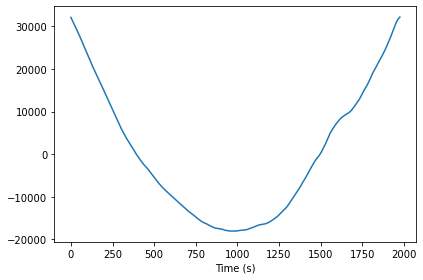
\includegraphics[width=0.8\linewidth]{signal_cumsum}
        \caption{Выходной сигнал}
        \label{fig:signal_cumsum}
    \end{figure}

    \begin{figure}[H]
        \centering
        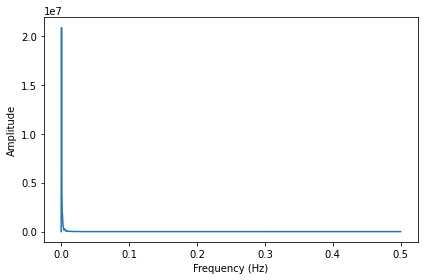
\includegraphics[width=0.8\linewidth]{signal_cumsum_spectrum}
        \caption{Спектр выходного сигнала}
        \label{fig:signal_cumsum_spectrum}
    \end{figure}

    Посмотрим на отношение входного и выходного сигнала.

    \begin{figure}[H]
        \centering
        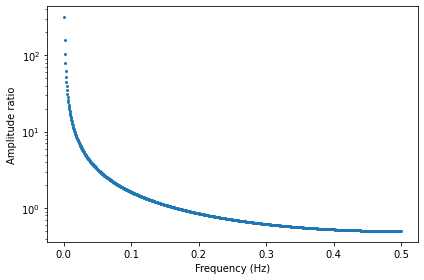
\includegraphics[width=0.8\linewidth]{in_out_ratio}
        \caption{Отношения входного и выходного сигнала}
        \label{fig:in_out_ratio}
    \end{figure}

    Построим фильтр для нарастающей суммы и сравним его с фильтром интегрирования.

    \begin{figure}[H]
        \centering
        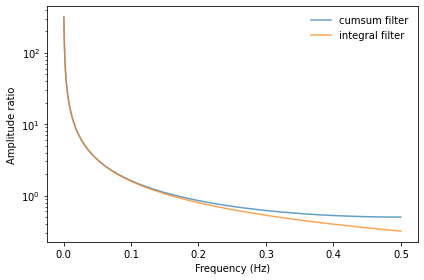
\includegraphics[width=0.8\linewidth]{cumsum_integr_diff}
        \caption{Фильтр нарастающей суммы и интегрирования}
        \label{fig:cumsum_integr_diff}
    \end{figure}

    На этой функции видно, что графики сначала совпадают, после расходятся.

    \begin{figure}[H]
        \centering
        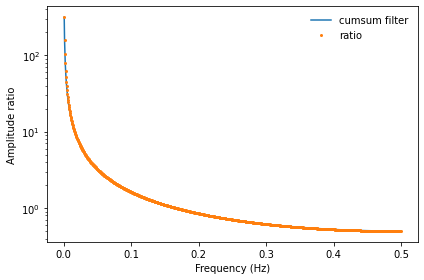
\includegraphics[width=0.8\linewidth]{ratio_filter_diff}
        \caption{Сравнение отношения и фильтра}
        \label{fig:ratio_filter_diff}
    \end{figure}

    Графики совпадают.
    Фильтр \texttt{cumsum} обратный фильтру \texttt{diff}.

    Применим \texttt{cumsum} в частотной области.

    \begin{figure}[H]
        \centering
        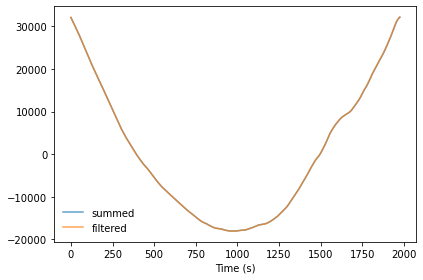
\includegraphics[width=0.8\linewidth]{cumsum_filter_diff}
        \caption{Сравнение суммирования и фильтрации}
        \label{fig:cumsum_filter_diff}
    \end{figure}

    Графики совпали.

    \newpage


    \section{Упражнение №2}
    \label{sec:2}

    В втором упражнении необходимо изучить влияние \texttt{diff} и \texttt{differentiate} на сигнал.
    Для этого необходимо создать треугольный сигнал, и применить у нему \texttt{diff}.
    Далее необходимо вычислить спектр сигнала, применить \texttt{differentiate} и посмотреть на результат.

    Создадим треугольный сигнал.

    \begin{lstlisting}[language=Python, caption= Создание треугольного сигнала, label={lst:make_triangle_signal}]
        from thinkdsp import TriangleSignal

        in_wave = TriangleSignal(freq=50).make_wave(duration=0.1, framerate=44100)
        in_wave.plot()
        decorate(xlabel='Time (s)')
    \end{lstlisting}

    \begin{figure}[H]
        \centering
        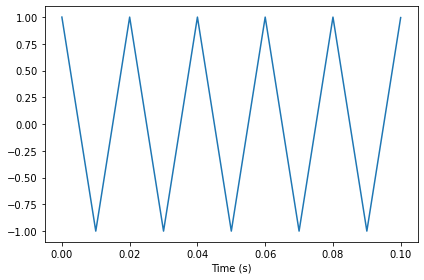
\includegraphics[width=0.8\linewidth]{triangle_signal}
        \caption{Треугольный сигнал}
        \label{fig:triangle_signal}
    \end{figure}

    Применим \texttt{diff} к сигналу.

    \begin{figure}[H]
        \centering
        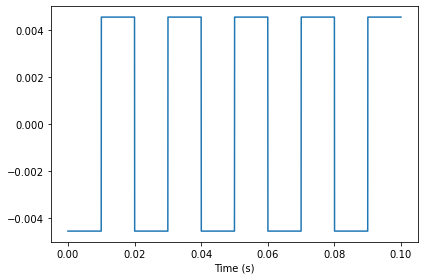
\includegraphics[width=0.8\linewidth]{triangle_diff}
        \caption{Результат применения diff к сигналу}
        \label{fig:triangle_diff}
    \end{figure}

    Вычислим спектр сигнала и применим к нему \texttt{differentiate}

    \begin{figure}[H]
        \centering
        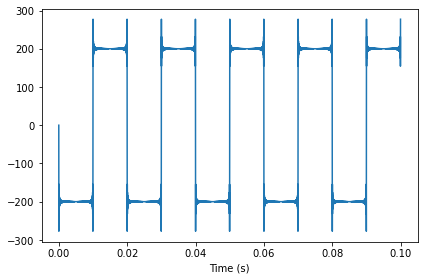
\includegraphics[width=0.8\linewidth]{triangle_differentiate}
        \caption{Результат применения differentiate к спектру сигнала}
        \label{fig:triangle_differentiate}
    \end{figure}

    На графике виден необычный эффект. Он вызван тем, что производная треугольного сигнала не определена в вершинах треугольника.

    \newpage


    \section{Упражнение №3}
    \label{sec:3}

    В третьем упражнении необходимо изучить влияние \texttt{cumsum} и \texttt{integrate} на сигнал.
    Для этого необходимо создать прямоугольный сигнал и применить к нему \texttt{cumsum}.
    Затем вычислить спектр сигнала и применить \texttt{integrate}.

    Создадим сигнал для дальнейшей работы.

    \begin{lstlisting}[language=Python, caption= Создание прямоугольного сигнала, label={lst:make_square_signal}]
        from thinkdsp import SquareSignal

        in_wave = SquareSignal(freq=50).make_wave(duration=0.1, framerate=44100)
        in_wave.plot()
        decorate(xlabel='Time (s)')
    \end{lstlisting}

    \begin{figure}[H]
        \centering
        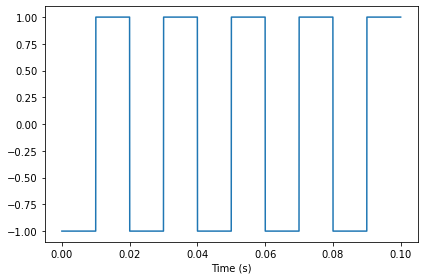
\includegraphics[width=0.8\linewidth]{square_signal}
        \caption{Прямоугольный сигнал}
        \label{fig:square_signal}
    \end{figure}

    Применим в полученному сигналу \texttt{cumsum}.

    \begin{figure}[H]
        \centering
        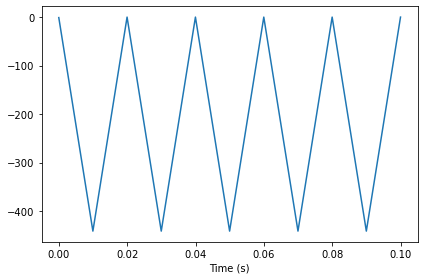
\includegraphics[width=0.8\linewidth]{square_cumsum}
        \caption{Результат cumsum}
        \label{fig:square_cumsum}
    \end{figure}

    Применим к спектру сигнала \texttt{integrate}

    \begin{lstlisting}[language=Python, caption= Применение integrate к спектру сигнала, label={lst:square_signal_spectrum_integrate}]
        spectrum = in_wave.make_spectrum().integrate()
        spectrum.hs[0] = 0
        out_wave2 = spectrum.make_wave()
        out_wave2.plot()
        decorate(xlabel='Time (s)')
    \end{lstlisting}

    \begin{figure}[H]
        \centering
        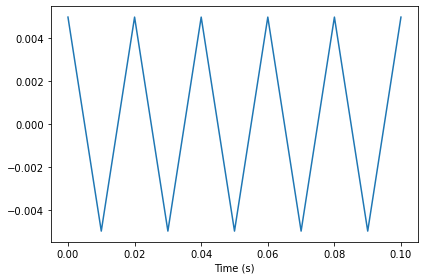
\includegraphics[width=0.8\linewidth]{square_integrate}
        \caption{Результат integrate}
        \label{fig:square_integrate}
    \end{figure}

    Результаты \texttt{cumsum} и \texttt{integrate} на вид получились одинаковыми.
    Проверим их схожесть.

    \begin{lstlisting}[language=Python, caption= Сравнение cumsum и integrate, label={lst:cumsum_integrate_compare}]
        out_wave.unbias()
        out_wave.normalize()
        out_wave2.normalize()
        out_wave.plot()
        out_wave2.plot()
    \end{lstlisting}

    \begin{figure}[H]
        \centering
        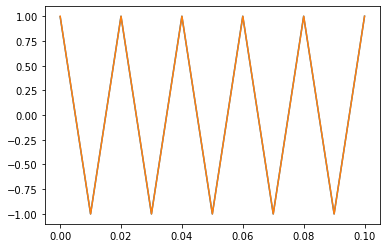
\includegraphics[width=0.8\linewidth]{cumsum_integrate_compare}
        \caption{Сравнение функций}
        \label{fig:cumsum_integrate_compare}
    \end{figure}

    По результатам видно, что различия в сигналах почти неразличимы.

    \newpage


    \section{Упражнение №4}
    \label{sec:4}

    В четвертом упражнении необходимо изучить влияние двойного интегрирования.
    Для этого надо создать пилообразный сигнал, вычислить его спектр и дважды применить \texttt{integrate}.

    Создадим пилообразный сигнал.

    \begin{lstlisting}[language=Python, caption= Создание пилообразного сигнала, label={lst:make_sawtooth_signal}]
        from thinkdsp import SawtoothSignal

        in_wave = SawtoothSignal(freq=50).make_wave(duration=0.1, framerate=44100)
        in_wave.plot()
        decorate(xlabel='Time (s)')
    \end{lstlisting}

    \begin{figure}[H]
        \centering
        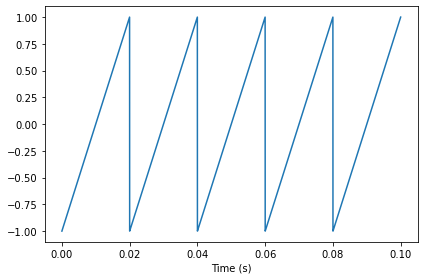
\includegraphics[width=0.8\linewidth]{sawtooth_signal}
        \caption{Пилообразный сигнал}
        \label{fig:sawtooth_signal}
    \end{figure}

    Применим двойное интегрирование к созданному сигналу.

    \begin{lstlisting}[language=Python, caption= Применение двойного интегрирования, label={lst:apply_double_integrate}]
        spectrum = in_wave.make_spectrum().integrate().integrate()
        spectrum.hs[0] = 0
        out_wave2 = spectrum.make_wave()
        out_wave2.plot()
        decorate(xlabel='Time (s)')
    \end{lstlisting}

    \begin{figure}[H]
        \centering
        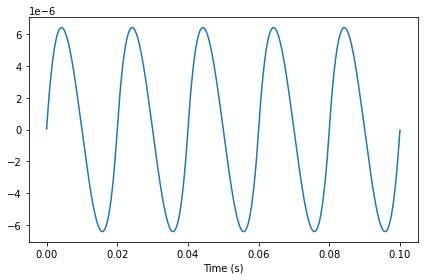
\includegraphics[width=0.8\linewidth]{sawtooth_double_integrate}
        \caption{Сигнал после двойного интегрирования}
        \label{fig:sawtooth_double_integrate}
    \end{figure}

    Создадим спектр сигнала после интегрирования.

    \begin{figure}[H]
        \centering
        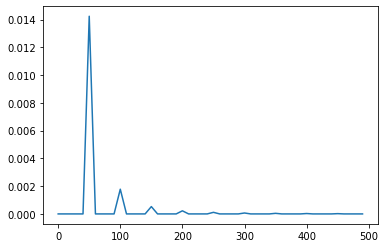
\includegraphics[width=0.8\linewidth]{sawtooth_integrate_spectrum}
        \caption{Спектр сигнала после интегрирования}
        \label{fig:sawtooth_integrate_spectrum}
    \end{figure}

    На графике видно, что сигнал напоминает синусоиду.
    Происходит это из-за того, что \texttt{integrate} действует как фильтр НЧ.
    На спектре видно, что отфильтровано все, кроме НЧ.

    \newpage


    \section{Упражнение №5}
    \label{sec:5}

    В четвертом упражнении необходимо изучить влияние второй разности и второй производной.
    Для этого надо создать \texttt{CubicSignal}, вычислить двойную разность применив \texttt{diff} и проанализировать результат.
    Далее вычислить вторую производную, дважды применив \texttt{differentiate} к спектру.

    Начнем с создания сигнала.

    \begin{lstlisting}[language=Python, caption= Создание кубического сигнала, label={lst:make_cubic_signal}]
        from thinkdsp import CubicSignal

        in_wave = CubicSignal(freq=0.0005).make_wave(duration=10000, framerate=1)
        in_wave.plot()
    \end{lstlisting}

    \begin{figure}[H]
        \centering
        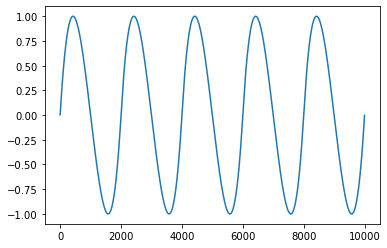
\includegraphics[width=0.8\linewidth]{cubic_signal}
        \caption{Кубический сигнал}
        \label{fig:cubic_signal}
    \end{figure}

    Вычислим двойную разность, дважды применив \texttt{diff}.

    \begin{figure}[H]
        \centering
        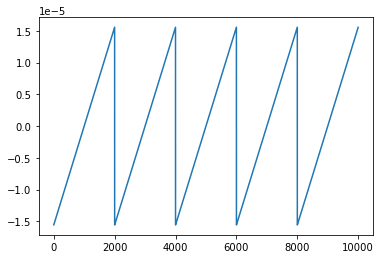
\includegraphics[width=0.8\linewidth]{cubic_double_diff}
        \caption{Вторая разность кубического сигнала}
        \label{fig:cubic_double_diff}
    \end{figure}

    Результат похож на пилообразный сигнал.

    Вычислим двойную производную, дважды применив \texttt{differentiate}.

    \begin{figure}[H]
        \centering
        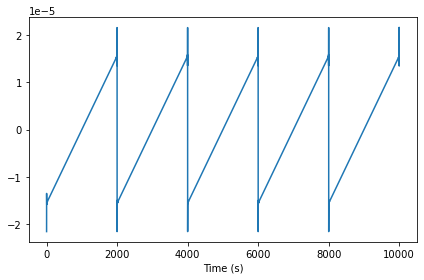
\includegraphics[width=0.8\linewidth]{cubic_double_differentiate}
        \caption{Вторая производная кубического сигнала}
        \label{fig:cubic_double_differentiate}
    \end{figure}

    Мы так же получили пилообразный сигнал с некоторым шумом.
    Связано это с тем, что производная параболического сигнала не определена в некоторых точках.

    Расчитаем фильтры, соответствующие второй разности и второй производной, и сравним их.

    \begin{figure}[H]
        \centering
        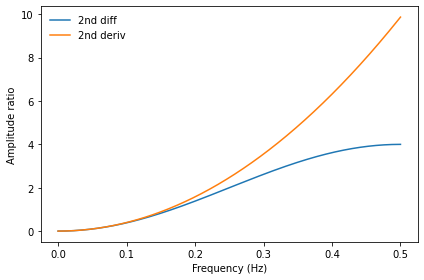
\includegraphics[width=0.8\linewidth]{double_filter}
        \caption{Сравнение фильтров}
        \label{fig:double_filter}
    \end{figure}

    Оба фильтра являются фильтрами ВЧ, которые усиливают компоненты наивысшей частоты.
    Поэтому на низких частотах различий нет, но на высоких становятся заметны.

    \newpage


    \section{Выводы}
    \label{sec:conclusions}

    В результате выполнения данной лабораторной работы были получены знания по интегрированию и дифференцированию сигналов.
    Была разобрана работа \texttt{diff}, \texttt{differentiate}, \texttt{cumsum} и \texttt{integrate}.
    Было изучено влияние двойного интегрирования, второй производной и второй разности на сигналы.

\end{document}